{
\setlength{\parindent}{2em}
\chapter{Flight Software Checkpointing}\label{cha:das-impl}
At its core, offering a suitable environment for the simulation of the flight software was the main purpose of the BBPSim simulator. Since \gls{SNC} wanted to reproduce the in-flight behavior of the communication sub-system as faithfully as possible, the software-in-the-loop test framework was designed according to the principle of encapsulation: exclude all internal changes to the simulated software and instead build around what is already there. Having said that, inevitably, there were exceptions made for some parts of the flight software algorithms, where code had to be altered to make it compatible to run on a Linux machine. For the most part, however, as shown in \autoref{fig:bbpsim-layers}, BBPSim succeeded in integrating \gls{DAS} as an "untouchable" nucleus and interfacing only indirectly with it.

The fact that DAS was supposed to stay completely permeable to modification forced the implementation of the save \& restore feature to treat it as a black box. This point of view brought several challenges, which were not present when modifying the BBPSim code to support checkpointing. 

In this section, the constraints that influenced the development of a checkpointing technique within the flight software are first of all described. It should be noted that most of the solutions to the problems were based on technical details that, in the end, had a meaningful impact. Subsequently, \gls{DAS} is briefly analyzed to clearly define which of its components' checkpointing are considered a necessary condition for a stable restore. Then, the approach taken to indirectly access, save and restore them is explained in details.

\section{Design Constraints}
It goes without saying that user and customer requirements play a big role in how the design goes forward. In particular, to make the \gls{FSW} checkpointable, it was important to bear in mind DCMS-BBP-121 (64-bit application), U02 (no alteration to FSW) and U01 (no instability). However, some other technicalities had a big importance too.

First and foremost, since the delivery method of BBPSim was through a Linux dynamic library, it was realized that most of the container-based solutions presented in \autoref{cha:state-of-the-art} could not apply to BBPSim. A shared object does not possess the same control than an application over many things, like memory layout. This presented a big problem, and a better explanation is given in the coming sections.

TO ADD HERE 

\section{Definition of Sufficient Condition for Restoration}
Saving and restoring an application was the main subject of \autoref{cha:state-of-the-art}. In every existing solution that was presented, the checkpointer programs did not have any control over the building process of the checkpointee. This made them approach the checkpointing problem from various angles, depending on the level at which the program was supposed to interact with the checkpointed application. 

In parallel, they each introduced a different sufficient condition, in terms of what to save, to be able to restore back the checkpointee. For example, it was considered essential for CRIU to save the totality of active memory pages inside the application's \gls{VMA} range, something pointless using the C\textsuperscript{3} environment.

Since the checkpointing feature of BBPSim was done with a different set of constraints, the set of necessary conditions for a stable restore had to once again be revisited. In this section, an assessment of the required components to checkpoint in the flight software is done. 

\subsection*{Definition of FSW Program State}
The description of requirement DCMS-BBP-122 on page \pageref{tab:customer-reqs} mentioned that "the current state of the [BBPSim] model" had to be saveable between steps. Undoubtedly, the word "model" is a very abstract term, and it could be interpreted in many ways. It was important to first define what qualified as a "model" in the more concrete context of DAS.

To better picture this, a parallel can be drawn with how C code is structured once compiled. When the \gls{GCC} compiles a valid C source file on Linux, an object file with extension \texttt{.o} is produced. Internally, this file is laid out in the Unix-wide standard \gls{ELF}. This very flexible format is divided into multiple segments that each have their own function in defining the program at low-level.

In this context, there are four relevant memory segments inside an object file:
\begin{wrapfigure}{r}{0.45\textwidth}
	\centering 
	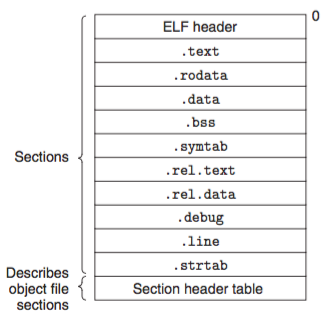
\includegraphics[width=.9\linewidth,keepaspectratio]{art/reloc-obj.png}
	\caption{Sections in an object file with ELF format.\cite{online:zhang}}
	\label{fig:sections-obj}
	\vspace{-24pt}
\end{wrapfigure}
\begin{enumerate}
	\item \textbf{\texttt{.bss}}. Contains the statically-allocated variables that were either uninitialized or initialized to zero.
	\item \textbf{\texttt{.data}}. Contains the statically-allocated variables that were initialized to zero.
	\item \textbf{\texttt{.text}}. Contains the binary instructions. Basically, the executable code.
	\item \textbf{\texttt{.rodata}}. Contains the read-only data (constants).
\end{enumerate}
\autoref{code:c-to-segments} shows how the translation is done using real C code.

In this thesis, it is argued that the state, or "model" of the flight software could be defined by two main components: the memory segments of statically-allocated variables, and the program counters. In the context of an object file, it was possible to redefine the state of a multithreaded DAS as being:
\begin{shadedquotation}
The full contents of the \texttt{.bss} and \texttt{.data} segments for all object files, the register set of each threads and the stack of each threads. 
\end{shadedquotation}

As for the \texttt{.rodata} and other segments, since they contain values that do not change from one simulation to the other, they were deemed unnecessary to include in this definition. Since they were identical at every simulation run, they were not included in the definition of the FSW state.

\subsection*{Condition 1 - Save Memory Segments}
The first necessary condition to be able to restore back to a previous "model" of DAS was to save the read-writeable, \textit{statically-allocated} regions in memory that concerned the flight software. It should be understood that a program's statically-allocated variables are variables that exist for the entire duration of the program. This term should not be confused with the \mintinline{c}|static| keyword of the C language, which limits the scope of a symbol in a compilation unit.

One can make an informal proof by contradiction of that statement by looking again at the sample code in \autoref{code:c-to-segments}. Let's suppose that, to restore DAS to a consistent global state, the restoration of the statically-allocated memory segments is not necessary. As a user, any changes done to variables (declared on lines \ref{lc-beg-statics} to \ref{lc-beg-statics}) during a simulation will be lost, and therefore, the global state of the application would not be consistent with the one on the previous run. Variables on the second run would not read the same as they would have at the end of the first one. The inclusion of these segments is thus a necessary condition.

\subsection*{Condition 2 - Save Register Sets}
A second necessary condition for a consistent DAS global state restore was to save the register set of every thread attached to the DAS program. In this set is located the \gls{PC}, depicted in \autoref{fig:x86-regs}. It is the CPU register in charge of keeping track of which instructions are to be executed. Since CPU instructions are encoded in binary and reside in the same \gls{VMA} as the variables, they are also addressable. In that sense, the program counter register holds the address of the current instruction being executed by the processor. One can think of the PC as being "where" the thread is in its execution of the program.

In addition, it was also important to save the other general-purpose registers, which contained the context of the CPU at that particular moment. Not putting the correct value in the registers would produce a domino effect resulting in a segmentation fault at best, or undefined behavior at worst.

\subsection*{Condition 3 - Save Thread Execution Stacks}
Finally, saving the thread execution stacks was considered the last necessary condition to make the checkpointing feature work in the context of the flight software. An execution stack contains a lot of very important information about the thread. For instance, the function-local (scoped) variables are located in this stack. For reasons similar to the first condition, it was also important to save them.

On top of that, even though the program counter represents the position of the execution of a thread at a certain time $t$, the stack also contains its \textit{backtrace}, information about the "path" taken by the thread to get there. Precisely, the backtrace (or stack trace) is defined as the series of functions that were called consecutively until $t$. The stack-related concepts are treated thoroughly in \autoref{sec:das-exec-restore}.

\subsection*{Building the Sufficient Condition}
When the three conditions listed above were grouped together, it was defined that this formed a sufficient condition for a consistent DAS global state restore. More formally, this thesis argues that:
\begin{itemize}
	\item with $F$ being a C function in DAS;
	\item with $G_s$ being the global state of DAS in memory;
	\item with $S_r$ being a previously saved state being restored;
\end{itemize}
then
\begin{equation} \label{eq:sr_equiv}
	\forall F: F(G_s)\equiv F(S_r)
\end{equation}
when $F$ is void of non-deterministic processes. All DAS functions satisfied to this criteria, because they were strictly exempt of dynamic memory allocation, random numbers, and scheduling non-determinism (since the order of execution for threads is set at compile-time).

It should be noted that \autoref{eq:sr_equiv} also holds true whether $F$ is \textit{stateful} or stateless (i.e whether calling $F$ with the same parameters yields the same output or not), since even function-scoped static variables are included in the memory segments that are part of a saved FSW state $S_r$. \autoref{code:c-to-segments} contains a good example of this. The \texttt{count()} function is stateful, but its state (i.e the value of \mintinline{c}|theCount|) is also included in the definition of the flight software state (in the \texttt{.bss} section).

Now that \textit{what} to save is properly defined, the following sections detail how the conditions were met for each of them in order to achieve a consistent checkpointing of the flight software.

\section{Black-box Symbol Access}\label{sec:das-mem-restore}
- Creation of the DAS state manager + symbol catalog
- how to access everything (talk about dynamic library loading, elf dumps, double linking etc.)
\section{Multithreaded Execution Backup and Restore}\label{sec:das-exec-restore}
When the program is executed, each section gets copied contiguously inside the virtual memory address range allocated for the program by the operating system. 
tried several techniques to save/restore execution stacks:
- sufficient conditions to be able to restore a task (w or w/o touching exec stack)
- different strategies, ultimately bounded by different reasons 
- strat 1 : just replay the thread until the first waitUntilNextPeriod() (there's 4 possible states : not created yet, created but not once had the "go", waiting in a waitUntilNextPeriod(), created but deleted)
- strat 2 : restart and stub functions, can do it with ELF-HOOK https://www.codeproject.com/Articles/70302/Redirecting-functions-in-shared-ELF-libraries
	Redirection of the OSApiWrapper calls, Extremely useful, because our library is a dynamic object, which means its calls to library functions are always resolved at runtime by looking in the .rel.plt (relocation, Procedure Linkage Table)
- strat 3 complicated version of longjmp: how to save execution (asm, disassembly of code, save sp, etc.% https://cs.brown.edu/courses/cs033/docs/guides/x64_cheatsheet.pdf)
Depends on the ABI

\subsection*{Shared Object Considerations}\label{sec:dynlib-considerations}
- Dynamic library loading  https://eli.thegreenplace.net/2011/08/25/load-time-relocation-of-shared-libraries
- address at which the library is loaded (why always 0x00007fffXXXXXXXX?) https://unix.stackexchange.com/questions/509607/how-a-64-bit-process-virtual-address-space-is-divided-in-linux
In this case, application continerization is not possible, because we are a library.

}